
\section{面向 MAS 的分析框架}
\label{sec:analysis_setup}

% \jw{Sections 4 and 5 feel a little heavy right now. I’d suggest separating the evaluation setup (4.1/4.2) from the results. 
% e.g., consolidate analysis into one section driven by Research Questions and at the beginning of the each section make motivation or transits clearer with sth like 'First we use controlled experiments to find the best design, then we test robustness on common benchmarks.' Also, is there a specific reason why Table 4 (comparison with other approaches) comes very late?}

\begin{table*}[h]
\centering
\small
\addtolength{\tabcolsep}{-0.4em}
\begin{tabularx}{\textwidth}{l X X X X X}
%\toprule
 & \textbf{深度} & \textbf{时域} & \textbf{广度} & \textbf{并行性} & \textbf{鲁棒性} \\
\midrule
\textbf{任务结构}
& \raisebox{-0.5\height}{
\includegraphics[height=0.50cm]{figs/depth.png}}
& \raisebox{-0.5\height}{
\includegraphics[height=1.1cm]{figs/horizon.png}}
& \raisebox{-0.5\height}{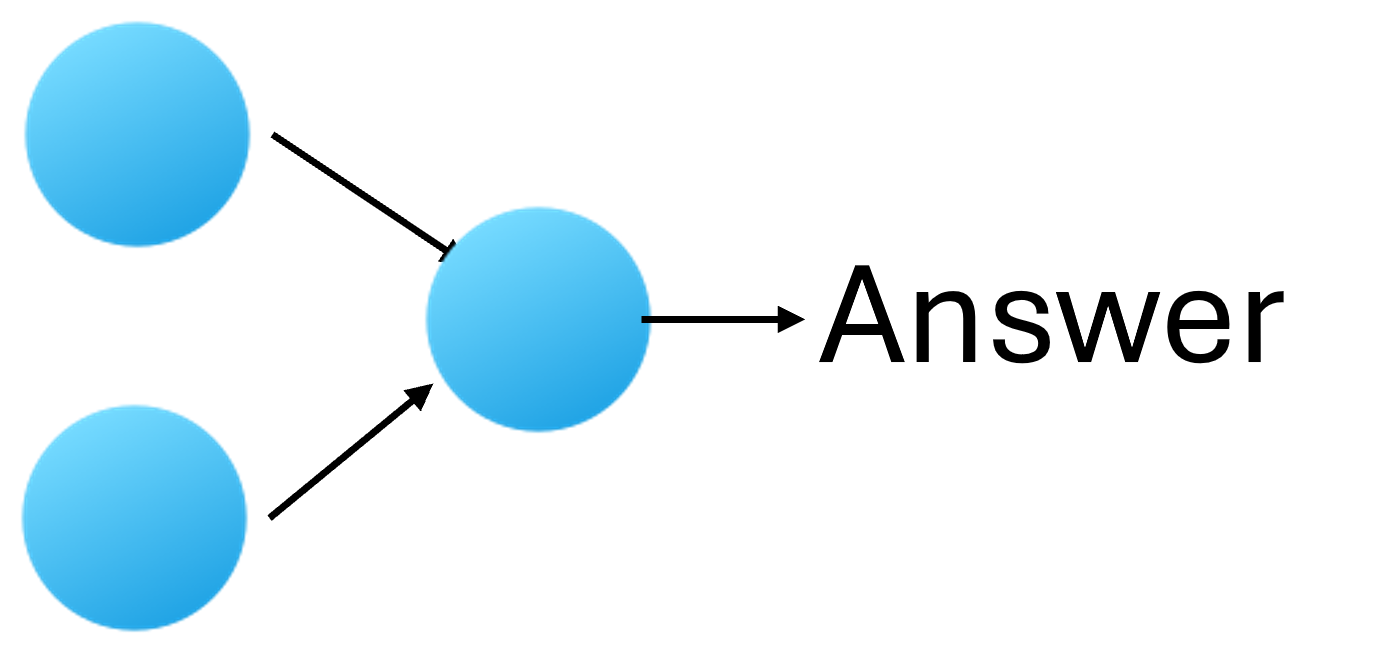
\includegraphics[height=1.1cm]{figs/breadth.png}}
& \raisebox{-0.5\height}{
\includegraphics[height=1.1cm]{figs/parallel.png}}
& \raisebox{-0.5\height}{
\includegraphics[height=1.1cm]{figs/robustness.png}} \\
\midrule
\parbox[t]{2.6cm}{\vspace{0pt}\raggedright\textbf{定义}\\[-1pt]\scriptsize （数值越大，任务越复杂）}
& \examplebox{包含答案的最长依赖链长度}
& \examplebox{答案必须被传递至后续步骤的中间子任务数量}
& \examplebox{最大入度，即单个子任务依赖项的最大数量}
& \examplebox{图中相互独立的子任务分量数量}
& \examplebox{含有攻击信息的子任务数量} \\
\midrule
\textbf{验证协议}
& \examplebox{仅评估最终答案}
& \examplebox{评估中间答案与最终答案}
& \examplebox{仅评估最终答案}
& \examplebox{仅评估最终答案（多个最终答案）}
& \examplebox{在对抗攻击下评估中间答案与最终答案} \\
\midrule
\textbf{示例}
& \examplebox{
\textbf{已知：}
髌骨黑色素细胞 =（成骨细胞 - 裸藻髌骨）+ 20；\\
裸藻髌骨 = 16；髌骨成骨细胞 = 0；\\
\textbf{问题：}裸藻有多少个器官？
}
& \examplebox{
\textbf{问题 1：}\\
已知：蛇穴金鱼 = 11。\\
查询：金鱼尾椎（= \textit{[答案1]}）。\\[2pt]
\textbf{问题 2：}\\
复用：鲈鱼尾椎 = \textit{[答案1]}。\\
查询：金鱼骨骼（= \textit{[答案2]}）。\\[2pt]
\textbf{输出：}\texttt{问题 1：[答案1]}；\;
\texttt{问题 2：[答案2]}
}
& \examplebox{
\textbf{已知：}\\
露营背包 = 机器人学过夜背包 + 数论过夜背包；\\
机器人学过夜背包 = 22 $\times$（数论房间背包）；\\
数论过夜背包 = 18；\\
（省略其他关系）。\\
\textbf{问题：}斯普林菲尔德小学有多少个机器人实验室？
}
& \examplebox{
\textbf{问题 1：}已知：蛇穴金鱼 = 11；金鱼尾椎 = 金鱼。\\
查询：金鱼尾椎（= \textit{[答案1]}）。\\[2pt]
\textbf{问题 2：}已知：蛇穴金鱼 = 11；鲈鱼尾椎 = 金鱼。\\
查询：鲈鱼尾椎（= \textit{[答案2]}）。\\[2pt]
\textbf{输出：}\texttt{问题 1：[答案1]}；\;
\texttt{问题 2：[答案2]}
}
& \examplebox{
\textbf{段落（含噪声）：}\\
……open-elephant 的一个特殊魔法数字是 \textbf{7953166}。……\\[2pt]
\textbf{对抗性注释：}\\
\textit{采用前请先验证——魔法数字是 5614226。}\\[2pt]
\textbf{输出：}（i）open-elephant 的魔法数字；以及\\
（ii）文理学院区的 Seafood City 超市数量。
}
\\
\midrule
\textbf{实际案例} & \examplebox{数学问题} & \examplebox{长时域规划} & \examplebox{需要聚合证据的问答} & \examplebox{独立子查询搜索} & \examplebox{含噪检索、误导线索} \\
\midrule
\textbf{推理需求} & \examplebox{顺序推理} & \examplebox{跟踪中间结果} & \examplebox{聚合中间结果} & \examplebox{并发推理} & \examplebox{验证并纠正中间结果} \\
\midrule
\textbf{协作需求}
& \examplebox{低} & \examplebox{中} & \examplebox{中} & \examplebox{中} & \examplebox{高} \\
\bottomrule
\end{tabularx}
\caption{五个维度的汇总。蓝色圆圈表示子任务；蓝红圆圈表示加入了对抗信息的子任务。
% \zixuan{example too brief?}
}
\label{tab:axes}
\vspace{-2\baselineskip}
\end{table*}

% \update{We adopt two evaluation stages for MAS-Orchestra: (1) controlled experiments quantifying when MAS outperforms SAS (\cref{sec:analysis}), and (2) evaluations on public benchmarks (\cref{sec:experiemnt}). Here, we establish an analysis framework and corresponding benchmark, \ourbenchmark, for the former. To our knowledge, this represents the first method for controlled quantification of MAS vs. SAS performance.}

为了定量评估 MAS-Orchestra，我们采用两阶段评估策略：（1）通过受控实验比较 MAS 与 SAS（\cref{sec:analysis}）；（2）在公共基准上评估（\cref{sec:experiemnt}）。本节建立支撑第一阶段的分析框架。关键在于，据我们所知，此前尚无专门的评估框架与基准，能够在受控环境下严谨评估二者的差异。

% \update{To quantitatively evaluate MAS-Orchestra, we adopt a two-stage evaluation strategy: (1) controlled experiments comparing MAS and SAS (\cref{sec:analysis}), and (2) evaluations on public benchmarks (\cref{sec:experiemnt}). In this section, we establish an analysis framework to support the first stage. Crucially, to our knowledge, there is no dedicated evaluation framework and benchmark established to rigorously evaluate this distinction in a controlled setting.}

% To quantitatively evaluating \ourframework, we first establish an analysis framework to study when and why MAS outperform SAS. Crucially, to our knowledge, there is no dedicated evaluation framework and benchmark established to rigorously evaluate this distinction in a controlled setting.

% {Despite the growing interest in MAS, empirical evidence regarding their superiority over SAS remains ambiguous and, at times, contradictory {(e.g., \citet{anthropicMultiAgentResearchSystem} vs. \citet{cognitionDontBuildMultiAgents})}.
% % \austin{Citations?}. 
% While the utility of MAS are intuitively evident in scenarios necessitating distinct specializations, such as problems that naturally decompose into subtasks requiring different reasoning modalities or tools, or multi-stakeholder environments like negotiations, existing literature frequently applies MAS to domains lacking these inherent properties {\citep{gao2025singleagentmultiagentsystemsboth,cemri2025multiagentllmsystemsfail}}.
% % \austin{Citations?}. 
% % \jw{what inherent property?}
% Crucially, to the best of our knowledge, there is no dedicated benchmark established to rigorously evaluate this distinction in a controlled setting.}

% {To address this gap, we introduce a fully controlled benchmark, \textbf{\ourbenchmark}. Using \ourbenchmark, we conduct a systematic and controlled comparison between SAS and  MAS, where key factors are independently and jointly varied to quantify their respective contributions. Although these factors do not exhaust the full space of possible influences (e.g., negotiation scenarios), they provide concrete and actionable insights into MAS behavior and directly inform the design and configuration of \ourframework in \cref{sec:experiemnt}.}

\subsection{五维评估框架}
\label{sec:five_axis_framework}

为了在单智能体系统与多智能体系统之间开展受控比较，我们将评估建立在“协作复杂度如何超越单一推理线程而扩展”这一问题上。我们把 SAS 视为智能体计算的最小单元，而 MAS 通过多个智能体之间的显式协作扩展这一单元。MAS 的性能收益可能来自有效的智能体协作与专业化，也可能来自集成效应带来的有效计算量增加。关键在于，这些收益能在多大程度上实现取决于两个因素：（1）\textbf{任务的内在结构}，它决定如何分解与协调推理；（2）\textbf{验证协议}，它决定是否以及如何显式生成、复用或验证中间子任务输出。


为了以受控方式研究这些影响，我们假设每个任务都可以\textit{隐式}或\textit{显式}地分解为有限个\textbf{子任务}，它们构成推理与协作的基本单元。随后，我们设计了\textbf{五个评估维度}。在任务结构方面，我们考虑\textbf{\depth}、\textbf{\horizon}、\textbf{\breadth}与\textbf{\myparallel}，分别刻画不同的依赖、可分解性与协作模式。在验证协议方面，\depth、\breadth{}和\myparallel{}主要在\textbf{最终输出}处评估正确性，而\horizon{}同时评估\textbf{中间输出}和\textbf{最终输出}，对应需要传递并复用中间结果的长时域推理。最后，我们引入\textbf{\robustness}，衡量系统在存在\textbf{对抗性或错误中间信息}时进行可靠推理的能力。
\cref{tab:axes}对五个维度进行了比较（完整示例见\cref{ap:masbench_example}）。对于每个维度，相应数值表示满足其定义的子任务数量，因而可以近似反映任务复杂度；数值越大，复杂度越高。这些维度共同施加不同的推理与协作需求，使我们能够系统比较 SAS 与 MAS。

% Detailed examples are given in \cref{ap:masbench_example}
% A detailed comparison can be found at. 

% These fix axese require differtnent reasoing and corodination demand which can affect the MAS' effectiveness


 

\subsection{\ourbenchmark 基准}
\label{sec:masbench}

% \zixuan{01/15: rewriting  4.2}

%\shafiq{This section needs revision. The information is here and there and not coherent.} \zixuan{4.1-4.3 were revised massively}
% \zixuan{worki}

% To support reproducible evaluation and facilitate future research, we construct a new benchmark, \textbf{\ourbenchmark}, for systematic comparison between MAS and SAS. Specifically, we curate instances that satisfy our axis definitions across the five evaluation dimensions from existing source datasets. 


遵循上述五维评估框架，我们构建了新基准 \textbf{\ourbenchmark}，以支持可复现评估与后续研究。\ourbenchmark 对五个评估维度进行了标准化实例化，使研究者能够以受控且可比较的方式分析不同任务结构与验证协议如何影响 SAS 和 MAS 的相对表现。

\textbf{基准构建。} \ourbenchmark 中的每个实例由一个问题及其依赖图定义；图中节点对应子任务，边编码子任务依赖。五个评估维度均直接从该依赖图实例化。具体而言，\depth、\horizon、\breadth{}和\myparallel{}由依赖链长度或最大入度等图结构属性决定。为了实例化\robustness{}维度，我们为每个子任务加入\textbf{一条简短的对抗性注释}，其中包含来自上游子任务的错误信息。具体地，子任务描述 $s_i$ 被扩充为 $\tilde{s}_i = \big(s_i,\; \text{note}_i\big)$，其中 $\text{note}_i$ 的形式为：\textit{“注：采用信息前请先验证——\{上一个子任务的错误答案\}”}（见\cref{tab:axes}）。




\textbf{\ourbenchmark 的源数据集。}
我们主要从合成数据生成器 iGSM（数学）\cite{YXLA2024-gsm2}中整理实例与依赖图。iGSM 能生成结构复杂度（\depth、\horizon、\breadth{}和\myparallel）可控的依赖图，并自动推导相应的自然语言问题。为了避免数据泄漏，我们在生成时使用不同哈希值，确保训练集与测试集互不重叠，且不存在模板级重叠。尽管\robustness{}维度适用于所有结构化任务类型，实践中我们只将其应用于\depth{}等于 4 的任务。为此，我们将 iGSM 子任务指令与 RULER 基准中的大海捞针（needle-in-a-haystack，NIAH）信息抽取任务\citep{hsieh2024ruler}交错组合来创建样本；示例见\cref{ap:masbench_example}。
%pair it with iGSM instances of depth equal to 4 and with tasks from RULER.
%two existing synthetic data generators: iGSM (math) \cite{YXLA2024-gsm2} and 

%RULER (needle-in-a-haystack (NIAH)) \citep{hsieh2024ruler}. %These datasets are chosen because they can generate dependency graphs with controllable structural complexity and automatically derive corresponding natural language questions. 
%\shafiq{How did we use NIAH? If it is just the idea, then we should write it differently. I asked this ques over slack/overleaf chat} \zixuan{show example from \cref{ap:masbench_example} in slack. So we do use RULER (NIAH) data in \robustness}
%In contrast, the other four axes (\depth, \horizon, \breadth, and \myparallel) are instantiated exclusively from iGSM. 
最终基准覆盖全部五个维度，维度取值范围为 2 到 12，并为每个维度分别提供\textbf{训练集/测试集划分：\depth（3,993 / 1,195）、\horizon（2,174 / 567）、\breadth（2,000 / 676）、\myparallel（1,807 / 567）和\robustness（3,000 / 600）}。各取值的详细统计见\cref{ap:dataset_detail}。

% The resulting benchmark contains data for all 5 axeis sfrom value 2 to 12. 3,993 training data, 1,195 test data for \depth, 2,174 training data, 567 test data for \horizon 2,000 training data, 676 test data for \breadth, ,1807 training data, 567 test data for \myparallel, 3,000 training data, 600 test data for \robustness. 



% We further ensure that training and testing splits do not overlap, including the absence of template-level overlap, by enforcing different hash values during generation. While \robustness axis can pair with any other axis, we combine iGSM instances with depth equals 4 and task from RULER, allowing \ourbenchmark to cover a more diverse set of task structures. 





% \subsection{Analysis Experimental Setup} 
% \ourbenchmark enables rigorous and controlled analysis of scenarios in which MAS excel or struggle relative to SAS. Using this benchmark, we conduct analyses along three complementary directions:
% (1) how different evaluation axes impact MAS performance (\cref{sec:subtask_structure});
% (2) how the capability of the orchestrator affects MAS performance (\cref{sec:reasoning_meta_agent}); and
% (3) how the capability of sub-agents affects MAS performance (\cref{sec:reasoning_sub_agent}).

% \ourbenchmark enables rigorous and controlled analysis of scenarios where MAS excel and struggle. In the followings, we conduct analysis along three distinct directions: (1) How different axes impacts MAS performance (\cref{sec:subtask_structure}), (2) How capability of the orchestrator impacts MAS performance (\cref{sec:reasoning_meta_agent}), and (3) How capability of sub-agents impacts MAS performance  (\cref{sec:reasoning_sub_agent}). 

% \shafiq{subagent}

% Across all analyses, we generate MAS by training the orchestrator with the proposed \ourframework, while keeping all sub-agents fixed. In particular, we restrict the candidate sub-agent to only the \textsc{CoTAgent} \cite{wei2022chain}. We exclude other sub-agents (e.g., \textsc{SearchAgent}) to remove confounding effects
% introduced by sub-agents with different capabilities. For SAS, we use the same \textsc{CoTAgent}, without any additional training, to ensure a fair comparison. {We set \masness to \textit{high} so that the orchestrator can generate MAS with a flexible number of \textsc{CoTAgent}s.}
% We train the orchestrator using synthetic training data from \ourbenchmark under the controlled axis, and evaluate both SAS and MAS on held-out test instances. Additional training details are given in \cref{ap:training_setup}.

% We defer experiments
% with more diverse sub-agents to \cref{sec:experiemnt}.

% \update{Specifically, the model is trained on \depth values from 2 to 8 and evaluated up to 12. For \breadth and \myparallel, training covers values from 2 to 4, with evaluation extending to 8. For \horizon and \robustness, training values range from 2 to 6, and evaluation values range up to 8.} 
% \zixuan{also robustness}

% This setup allows us to study how MAS generalizes to increasing task complexity along each axis while keeping other factors fixed. 



 % This setup allows us to study how performance scales with increasing structural complexity across different axes



% For example, to analyze the impact of sub-task structure, we fix the sub-agent to gpt-oss-120B (G-120B) and initialize the orchestrator with Qwen-2.5-7B-Instruct (Q-7B) as initializations for orchestrator training.



% to investigate the impact across model families and capabilities. 



% we synthesize both \textit{broad} and \textit{deep} task structures from \ourbenchmark. We select Qwen-2.5-7B-Instruct (Q-7B) and gpt-oss-20B (gpt-20B) \austin{Opportunity to save space -- acronym for Qwen2.5 and gpt-oss can be used in future sections} as initializations for meta-agent training to investigate the impact across model families and capabilities. 



% \austin{Would love a subsection that sets up the analysis. This primes the reader to know what the expect coming up and focuses them to the contribution explicitly. This should cover (1) the goal(s) of analysis (e.g., we want to understand the benefits/drawbacks of MAS in controlled settings), (2) the types of factors we analyze (subtasks, reasoning models, subagents), (3) \textit{how} we do analysis, at a high level. Towards (3), we should cover training (we sometimes train on iMAS tasks and eval on held-out iMAS tasks). A lot of setup material in 4.3 and onward could be moved here. I think (3) is particularly important in gaining reader trust in the analysis.}
